\chapter{Analyse}
\label{sec:analyse}
Dieses Kapitel der Arbeit betrachtet zunächst den gegenwärtigen Stand der Technik hinsichtlich bereits vorhandenen Tools. Ihre Stärken und Schwächen werden ebenfalls aufgezeigt. Danach geht es um die Anforderungsanalyse der Webanwendung. Dazu wird eine allgemeine Struktur festgelegt, wie die Arbeit systematisch aufgebaut sein soll. Anschließend wird der aktuelle Zustand (Ist-Analyse) des Projektes ermittelt und anhand dieser Ist-Analyse erfolgen die funktionalen und nicht-funktionalen Anforderungen an die zu entwickelnde Webanwendung.

\section{Stand der Technik}
\label{sec:stand der technik}
Bei der Suche nach öffentlich zugänglichen Tools für die Durchführung von Workshops wurden folgenden Ergebnisse gefunden:

\subsection{IdeaBoardz}
\label{sec:ideaBoardz}
IdeaBoardz\footnote{vgl. \url{https://ideaboardz.com/}} ist eine freie webbasierte Anwendung zum Brainstorming, Erstellen einer ToDo-Liste oder zur Retrospektive im agilen Projektmanagement. Mit diesem Tool ist eine Zusammenarbeit möglich. Die beteiligten Personen können entweder zeitgleich oder zu verschiedenen Zeiten ortsunabhängig auf das gemeinsame Dokument zugreifen und bearbeiten. In Echtzeit zusammenarbeiten, ist bei IdeaBoardz nicht realisierbar. Das hat zur Folge, dass bei der Veränderung des Zustands keine sofortige Aktualisierung der Benutzeroberfläche erfolgt. IdeaBoardz wird unter anderem bei Brainstorming-Methode wie die 6-Hüte-Methode\footnote{engl. Six Thinking Hats} von De Bono und auch für die Ideenbewertung bekannte SWOT\footnote{steht für Strengths-Weaknesses-Opportunities-Threats-Analyse}-Analyse angewendet. Die Registrierung ist optional, so dass der Nutzer auch IdeaBoardz verwenden kann, ohne sich anzumelden.

\begin{figure}[H]
  \begin{center}
    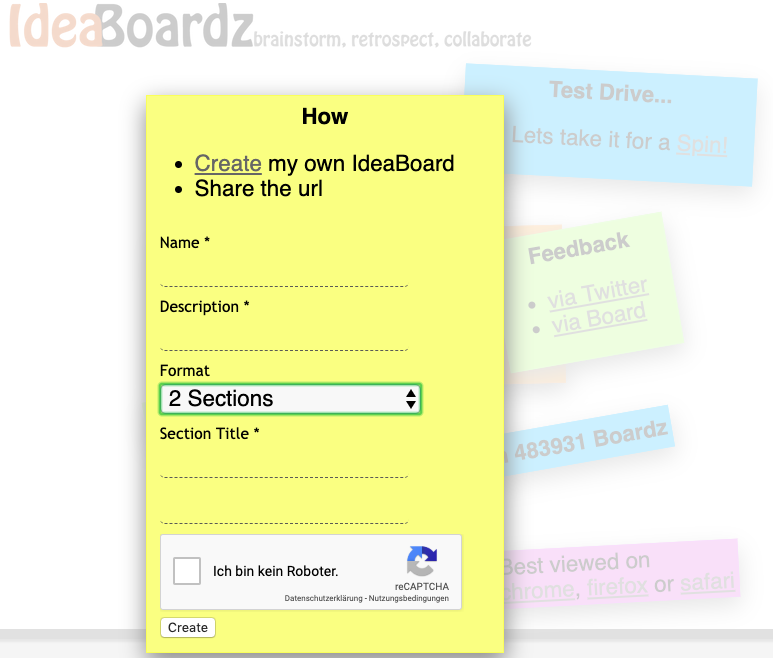
\includegraphics[scale=0.3]{img/ideaBoardz1}
	\caption{Erstellen eines eigenen IdeaBoards.} 
	\label{fig:erstellen des eigenen ideaboards}
  \end{center}   
\end{figure}

Die \textbf{Abbildung \ref{fig:erstellen des eigenen ideaboards}} zeigt, wie ein IdeaBoard zu erstellen ist. Neben dem Namen des Boards werden das Thema (Description) und Formate (Format) benötigt. Es können bis zu 10 Sektionen gewählt werden und es stehen noch weitere Formate zur Verfügung, wie Pro und Contra, ToDo-Liste, Six Thinking Hats und vieles mehr. Anschließend wird ein Titel für jegliche Sektionen eingegeben.

\begin{figure}[H]
  \begin{center}
    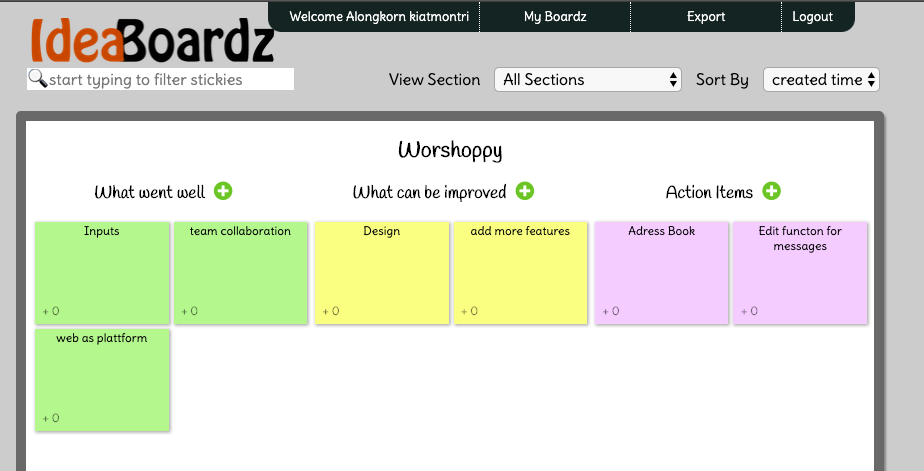
\includegraphics[scale=0.35]{img/ideaBoardz2}
	\caption{Darstellung von Sektionen} 
	\label{fig:darstellung von sektionen}
  \end{center}   
\end{figure}

Wie in \textbf{Abbildung \ref{fig:darstellung von sektionen}} zu sehen ist, sind die Eingaben in Sektionen strukturiert und farbig sortiert. Das Thema steht in der Mitte. Jede Sektion hat einen Titel und einen Plus-Button. Mit diesem Button können zu jeder Sektion neue Eingaben hinzugefügt werden. Die Eingaben werden als Karteikarten bzw. Notizzetteln visualisiert. Der weiße Hintergrund kann wie ein Whiteboard oder eine Pinnwand gesehen werden. Die Eingaben können auch von beteiligten Personen abgestimmt werden. Es ist auch möglich, die Daten nach Datum oder Abstimmung sortieren zu lassen.\bigskip

Als weiteres Feature lassen sich die Sektionen einzeln darstellen (\textbf{Abbildung \ref{fig:darstellung einer der sektionen}}). Die Suche nach dem Eingabeinhalt und das Exportieren der Ergebnisse sowohl als PDF-Datei als auch in ein Excel-Dokument werden ebenfalls bei dieser Webanwendung angeboten. Die Daten können sowohl innerhalb als auch außerhalb der Sektion zusammengeführt (Merge) werden. Ebenso lassen sich die Daten aus einer Sektion anderer Daten per Drag \& Drop zuordnen, wie in \textbf{Abbildung \ref{fig:zusammenführen und zuordnen von daten}} zu sehen ist. Mit dem Teilen von URL kann das jeweilige IdeaBoardz für die Zusammenarbeit freigegeben werden.

\begin{figure}[H]
  \begin{center}
    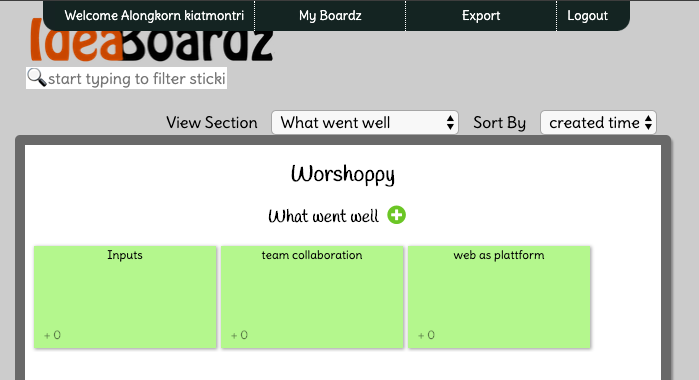
\includegraphics[scale=0.4]{img/ideaBoardz3}
	\caption{Darstellung einer der Sektionen} 
	\label{fig:darstellung einer der sektionen}
  \end{center}   
\end{figure}

\begin{figure}[H]
  \begin{center}
    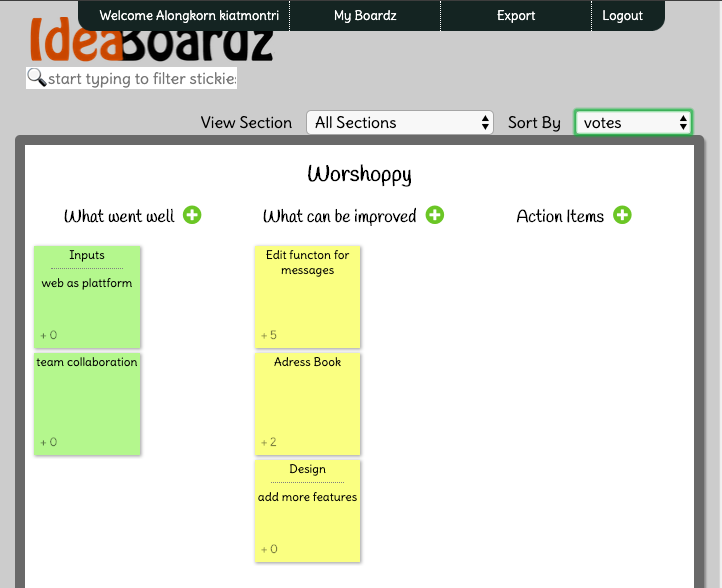
\includegraphics[scale=0.35]{img/ideaBoardz4}
	\caption{Zusammenführen und Zuordnen von Daten} 
	\label{fig:zusammenführen und zuordnen von daten}
  \end{center}   
\end{figure}

\newpage
Einige der oben dargestellten Features können für das Workshoppy-Projekt übernommen werden. Zu nennen sind:

\begin{itemize}
\item Die Eingabe wie ein Notizzettel oder Karteikarten visualisieren.
\item Die Ergebnisse als PDF-Datei exportieren.
\item Eingaben in Sektion darstellen.
\item Zuordnung von Daten (per Drag \& Drop).
\end{itemize}

Mit welchen Webtechnologien IdeaBoardz entwickelt wurde, lässt sich anhand der Informationen auf der Webseite nicht erkennen. Man kann aber davon ausgehen, dass es sich bei IdeaBoardz um eine webbasierte Anwendung mit reichlich Interaktionen auf der Benutzeroberfläche handelt, d.h. es ist über einen Webbrowser nutzbar und der Nutzer muss nichts installieren. Dementsprechend gehört IdeaBoardz zu einer Thin Client-Anwendung und zählt auch zu Rich Internet Applications sowie Web 2.0-Anwendung. (\textbf{siehe Kapitel \ref{sec:grundlagen}}).

\subsection{Miro-RealtimeBoard}
\label{sec:miro-realtimeBoard}
Miro\footnote{vgl. \url{https://miro.com/}} ist eine dynamische Webanwendung und handelt es sich um ein kollaborativer Online-Whiteboard in Echtzeit. Um das Online-Whiteboard nutzen zu können, wird ein Account benötigt. Dafür muss man sich bei Miro registrieren. Miro bietet die kostenlose Version an, sie ist für bis zu drei Teammitglieder und drei Boards geeignet.\bigskip

Begonnen wird mit einer leere Seite oder man verwendet eine von Miro bereitgestellten Vorlage. Zur Vorlage gehören unter anderem MindMap, Flowchart, Brainwriting und Concept Map. Einfügen neuer Dateien, Bilder und Dokumenten aus Google Drive oder vom Rechner ist auch möglich, um Informationen auszutauschen. Der Nutzer kann virtuelle Notizen erstellen. Die Notizen können sich nach Farbe unterscheiden und per Drag \& Drop über das komplette Board verschieben. Mit Hilfe von Share-Button vereinfacht Miro die Teilen-Funktion über eine URL oder einen Gmail-Account das ortsunabhängige und kollaborative Arbeiten in Echtzeit. Somit können die beteiligten Person beispielsweise während des Brainstormings auf die Ideen der anderen eingehen und kommentieren. Außerdem können die Benutzer das Whiteboard in eine Präsentation umwandeln oder als eine PDF-Datei exportieren.\bigskip

Miro ist ebenfalls gut geeignet zur Umsetzung eines klassischen Brainstormings (\textbf{Abbildung \ref{fig:miro board}}). Die Ideen werden in Form von Notizen erstellt. Zusammenfassend können die Notizen nach Farben kategorisiert werden.  

\begin{figure}[H]
  \begin{center}
    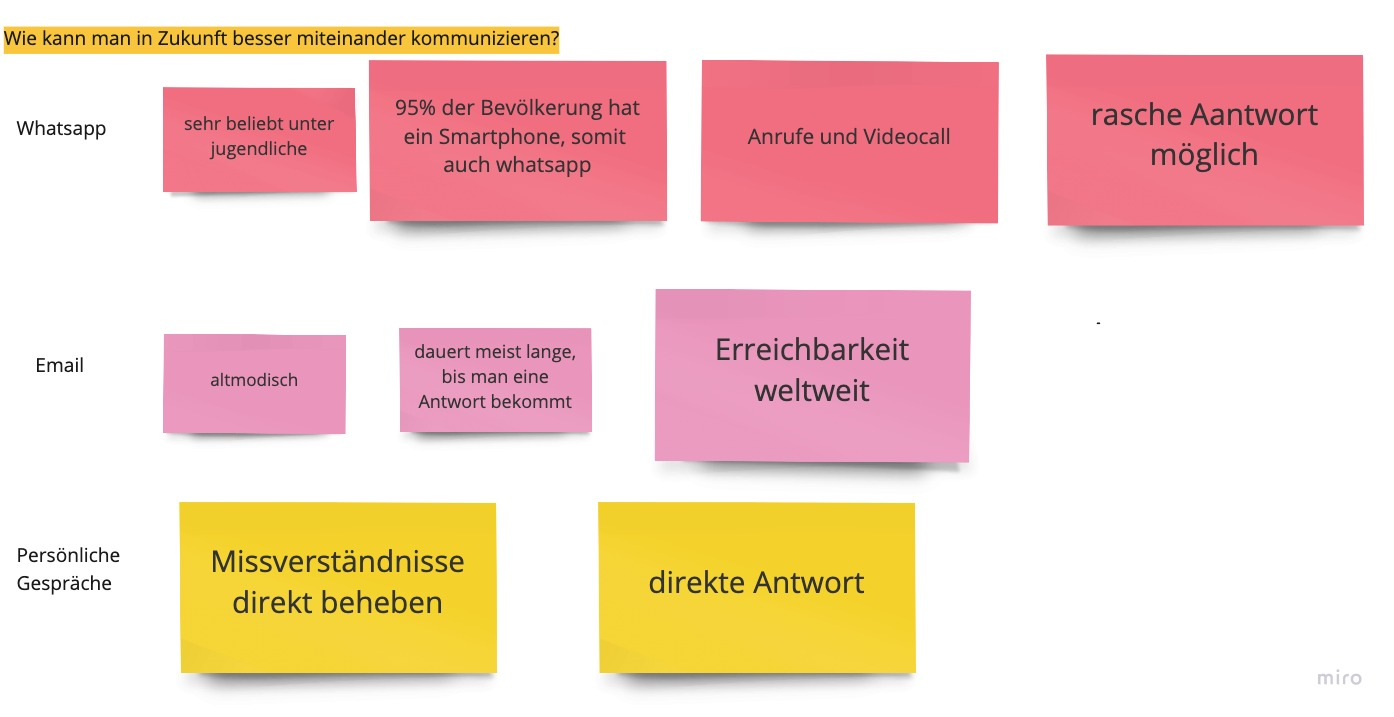
\includegraphics[scale=0.25]{img/miro1}
	\caption{Realisieren eines Brainstormings mit Hilfe von Miro} 
	\label{fig:miro board}
  \end{center}   
\end{figure}

Folgende Erkenntnisse wurden bei der Analyse von Miro gefunden und werden für das Workshoppy-Projekt übernommen: 
\begin{itemize}
\item AJAX-Anwendung
\item Thin Client-Anwendung
\item Web 2.0-Anwendung
\item Rich Internet Applications
\end{itemize}

\subsection{MindMap}
\label{sec:mindmap}



